% This text is proprietary.
% It's a part of presentation made by myself.
% It may not used commercial.
% The noncommercial use such as private and study is free
% Sep. 2005 
% Author: Sascha Frank 
% University Freiburg 
% www.informatik.uni-freiburg.de/~frank/

\documentclass{beamer}
\usepackage{multicol}
\usepackage{amsmath}

\usepackage{tikz}
\usetikzlibrary{shapes.geometric, arrows, positioning}

\usetheme{Warsaw}

\begin{document}
\title{Public key cryptology, RSA, ElGamal, Elliptic Curve}   
\author{Jason Pearson and } 
\date{\today} 

\frame{\titlepage} 

\frame{\frametitle{Key Terms}
	Plain text: typically a simple text such as this line \newline
	Cipher text: a message after it has been encrypted \newline
	Prime Number: a whole number that can only be divided evenly by one and itself also it is greater than one \newline
	
}
\frame{\frametitle{Types of Encryption}
	Symmetric Encryption \newline
	Asymmetric Encryption \newline
	Hashing \newline
	Hybrid Encryption \newline
}

\frame{\frametitle{Symmetric Encryption}
	Encryption and Decryption use the same key\newline
	
	\center
	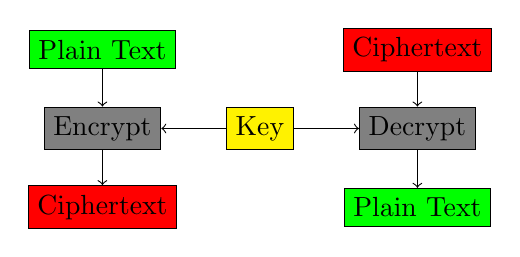
\begin{tikzpicture}[node distance=2cm]
	\node[draw, fill=green] (plainOne) at (0,2) {Plain Text};
	\node[draw, fill=gray] (encrypt) at (0,1) {Encrypt};
	\node[draw, fill=red] (cipherOne) at (0,0) {Ciphertext};
	\node[draw, fill=yellow] (key) at (2,1) {Key};
	\node[draw, fill=red] (cipherTwo) at (4,2) {Ciphertext};
	\node[draw, fill=gray] (decrypt) at (4,1) {Decrypt};
	\node[draw, fill=green] (plainTwo) at (4,0) {Plain Text};
	
	\draw[->,draw=black] (plainOne) to (encrypt);
	\draw[->,draw=black] (encrypt) to (cipherOne);
	\draw[->,draw=black] (key) to (encrypt);
	\draw[->,draw=black] (key) to (decrypt);
	\draw[->,draw=black] (cipherTwo) to (decrypt);
	\draw[->,draw=black] (decrypt) to (plainTwo);
	\end{tikzpicture}
	
}
\frame{\frametitle{Asymmmetric Encryption}
	Public key and private key pair \newline
	Public key is used to encrypt a message\newline
	Private key is used to decrypt a message\newline
	Creating the key tends to be computationally expensive\newline
	
	\center
	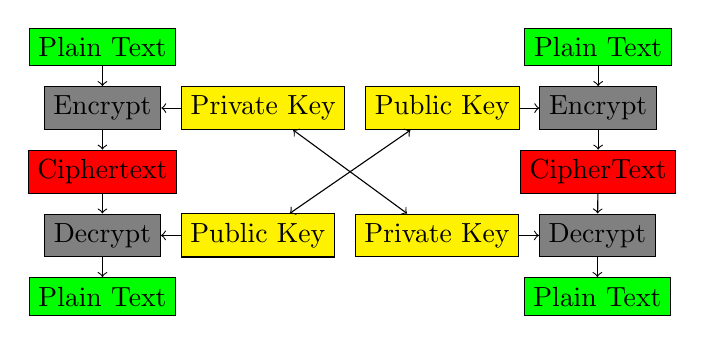
\begin{tikzpicture}[node distance=.25cm]
		\node[draw, fill=green] (plainOne) {Plain Text};
		\node[draw, fill=gray, below = of plainOne] (encryptpriv) {Encrypt};
		\node[draw, fill=red, below = of encryptpriv] (cipherOne) {Ciphertext};
		\node[draw, fill=yellow, right = of encryptpriv] (keypriv) {Private Key};
		\node[draw, fill=gray, below = of cipherOne] (decryptpub)  {Decrypt};
		\node[draw, fill=green, below = of decryptpub] (plainTwo) {Plain Text};		
		\node[draw, fill=yellow, right = of decryptpub] (keypub)  {Public Key};
	
		\node[draw, fill=yellow, right = of keypriv] (keypubtwo) {Public Key};
		\node[draw, fill=yellow, right = of keypub] (keyprivtwo) {Private Key};
		\node[draw, fill=gray, right = of keypubtwo] (encryptpub) {Encrypt};
		\node[draw, fill=gray, right = of keyprivtwo] (decryptpriv) {Decrypt};
		\node[draw, fill=green, below = of decryptpriv] (plainFour) {Plain Text};
		\node[draw, fill=green, above = of encryptpub] (plainThree) {Plain Text};
		\node[draw, fill=red, below = of encryptpub] (cipherThree) {CipherText};
		
		
		\draw[->,draw=black] (plainOne) to (encryptpriv);
		\draw[->,draw=black] (encryptpriv) to (cipherOne);
		\draw[->,draw=black] (keypriv) to (encryptpriv);
		\draw[->,draw=black] (cipherOne) to (decryptpub);
		\draw[->,draw=black] (keypub) to (decryptpub);
		\draw[->,draw=black] (decryptpub) to (plainTwo);
		
		\draw[->,draw=black] (plainThree) to (encryptpub);
		\draw[->,draw=black] (encryptpub) to (cipherThree);
		\draw[->,draw=black] (keypubtwo) to (encryptpub);
		\draw[->,draw=black] (cipherThree) to (decryptpriv);
		\draw[->,draw=black] (keyprivtwo) to (decryptpriv);
		\draw[->,draw=black] (decryptpriv) to (plainFour);
		
		\draw[<->, draw=black] (keypub) to (keypubtwo);
		\draw[<->, draw=black] (keypriv) to (keyprivtwo);
		
	\end{tikzpicture}
}


\frame{\frametitle{Hashing}
	We may or may not want to talk about this?
	
}



\frame{\frametitle{Hybrid Encryption}
	Uses ideas from symmetric and asymmetric encryption methods \newline
	An asymmetric cryptosystem is used for key encapsulation and an symmetric system is used for data encapsulation\newline
	
		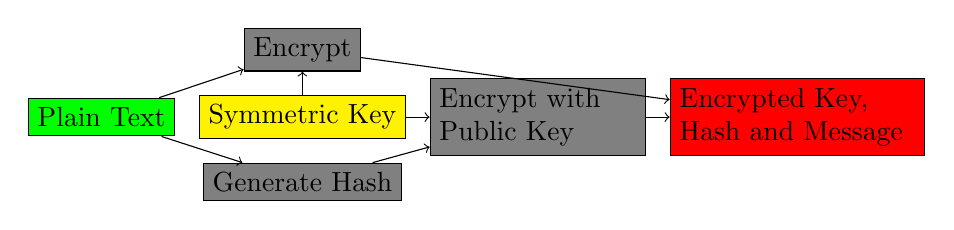
\begin{tikzpicture}[node distance=.3cm]
		\node[draw, fill=gray] (encrypt) {Encrypt};
		\node[draw, fill=yellow, below = of encrypt] (symkey) {Symmetric Key};
		\node[draw, fill=gray, below = of symkey] (hash) {Generate Hash};
		\node[draw, fill=green, left = of symkey] (plaintext) {Plain Text};
		\node[draw, fill=gray, right = of symkey, text width = 2.5cm] (encryptpub) {Encrypt with Public Key};
		\node[draw, fill=red, right = of encryptpub, text width = 3cm] (asymencrypt) {Encrypted Key, Hash and Message};
		
		
		\draw[->,draw=black] (plaintext) to (encrypt);
		\draw[->,draw=black] (plaintext) to (hash);
		\draw[->,draw=black] (hash) to (encryptpub);
		\draw[->,draw=black] (symkey) to (encrypt);
		\draw[->,draw=black] (symkey) to (encryptpub);
		\draw[->,draw=black] (encrypt) to (asymencrypt);
		\draw[->,draw=black] (encryptpub) to (asymencrypt);
		
		\end{tikzpicture}
}

\frame{\frametitle{Padding Schemes}
	
}

\frame{\frametitle{RSA Cryptosystem}
	First designed in 1973 and declassified in 1997. \newline
	Named after its founders Ron Rivest, Adi Shamir and Leonar Adleman \newline
	Uses large prime numbers to create a private and public key \newline
	Security arises from the presumed difficulty of factoring large prime numbers \newline
}

\frame{\frametitle{RSA Generating Public and Private Keys}
	Generate two large prime numbers and use to calculate n\newline
	Compute Euler's Totient Function \newline
	Create Public Key and Private Key \newline
}


\frame{\frametitle{Generating Large Prime Numbers}
	Generate two large prime numbers. \newline
	Typically uses AKS testing and/or the Miller-Rabin test for prime numbers \newline
	These two values we will call p and q \newline
	p = 991 \newline
	q = 821 \newline
	We next calculate n = p * q \newline
	So we have n = 991 * 821 = 813611 \newline
	
	\begin{center}
		\begin{tabular}{| c | c |}
			\hline
			Public Information & Secret Information\\ \hline
			n = 813611 & q = 821  \\ \hline
			 & p = 991 \\ \hline
		\end{tabular}
	\end{center}
}

\frame{\frametitle{Euler's Totient}
	We then can determine Euler's totient value by using the following equation. \newline
	$\phi \left(n\right)=\phi \left(p\right)\phi \left(q\right)=\left(p-1\right)\left(q-1\right)=n-\left(p+q-1\right)$ \newline
	And for $\phi \left( n \right) = \phi \left( 813611 \right) = 811800$ \newline
	
		\begin{center}
			\begin{tabular}{| c | c |}
				\hline
				Public Information & Secret Information\\ \hline
				n = 813611 & q = 821  \\ \hline
				 & p = 991 \\ \hline
				 & $\phi \left(n\right)$  = 811800\\ \hline
			\end{tabular}
		\end{center}
	
}

\frame{\frametitle{Create Public and Private Keys}
	To create a public key we pick an arbitrary number e between $1 < e < \phi \left(n\right)$ for example we will use e = 7423 \newline
	To create a private key we need to find the modular multiplicative inverse of e. \newline 
	This is commonly done using the Extended Euclidean Algorithm. \newline
	
	$d\equiv {e}^{-1}\left(\mathrm{mod}\left(\phi \left(n\right)\right)\right)$ \newline
	This makes our value of d = 788287 
	\begin{center}
		\begin{tabular}{| c | c |}
			\hline
			Public Information & Secret Information\\ \hline
			n = 813611 & q = 821  \\ \hline
			e = 7423  & p = 991 \\ \hline
			 & $\phi \left(n\right)$  = 811800\\ \hline
			  & d = 788287 \\ \hline
		\end{tabular}
	\end{center}
	
}

\frame{\frametitle{Working Example}
	Using these values we can create a cipher text c and decrypt it using the following equations \newline
	$c\equiv {m}^{e}\left(mod\left(n\right)\right)$ and
	$m\equiv {c}^{d}\left(mod\left(n\right)\right)$ \newline
	Finishing up our example we will encrypt "Hi" using our new values \newline
	plain text m = 72105, e = 7423, d = 788287, n = 813611\newline
		\begin{center}
			\begin{tabular}{| c | c |}
				\hline
			Public Encrypt & Private Encrypt \\ \hline
			$c\equiv {m}^{e}\left(mod\left(n\right)\right)$ & $c\equiv {m}^{d}\left(mod\left(n\right)\right)$ \\ \hline
			$c \equiv {72105}^{7423} mod (813611)$ & $c \equiv {72105}^{788287} mod (813611)$ \\ \hline
			$c = 707473$  & $c = 616895$ \\ \hline \hline
			Private Decrypt & Public Decrypt \\ \hline
			$m\equiv {c}^{d}\left(mod\left(n\right)\right)$ & $m\equiv {c}^{e}\left(mod\left(n\right)\right)$ \\ \hline
			$m \equiv {707473}^{788287} mod (813611)$ & $m \equiv {616895}^{7423} mod (813611)$\\  \hline
			$m = 72105$ & $m = 72105$\\ \hline
			\end{tabular}
		\end{center}
}


\frame{\frametitle{RSA Practical Usage}
	
}


\frame{\frametitle{ElGamal Cryptosystem}
	This method for cryptogphy uses discrete logarithms with a large prime modulus \newline
	The first step in creating is to create a large prime number \newline
	Then we create a Public and Private key \newline
	These can be used to encrypt and decrypt information \newline
}

\frame{\frametitle{Generating Large Prime Numbers}
	First we generate a large prime number p\newline
	For us p = 17 \newline
	We then create a generator g of multiplicative group $ \mathbb{Z}_{p}^{*}$ of integers modulo p \newline
	For this example g = 6 \newline
	\begin{center}
		\begin{tabular}{| c | c |}
			\hline
			Public Information & Private Information \\ \hline
			p = 17 & \\ \hline
			g = 6 & \\ \hline
		\end{tabular}
	\end{center}
}


\frame{\frametitle{ElGamal Creating Public and Private Keys}
	We then select a private key a where $1\le a\le p-2$ \newline
	For this example a = 5 \newline
	We can then use this to generate the last part of the public key \newline ${g}^{a}\mathrm{mod}p = {6}^{5}\mathrm{mod}17 = 7$
		\begin{center}
			\begin{tabular}{| c | c |}
				\hline
				Public Information & Private Information \\ \hline
				p = 17 & a = 5\\ \hline
				g = 6 & \\ \hline
				${g}^{a}\mathrm{mod}p$ = 7 & \\ \hline
			\end{tabular}
		\end{center}
}

\frame{\frametitle{Encrypting a Message}
	We will have our message m = 13 \newline
	A public sender to send a message to the private key holder picks a random value k for this example k = 10\newline
	We then compute $c_{1}={g}^{k} mod p = 15$ \newline
	Now $c_{2}= m * {g}^{k}\mathrm{mod}p= 13 * {6}^{10}  mod 17 = 8$ \newline
	Cipher text sent through $c_{1}$ and $c_{2}$ to private key holder \newline
	\begin{center}
		\begin{tabular}{| c | c |}
			\hline
			Public Information & Private Information \\ \hline
			p = 17 & a = 5\\ \hline
			g = 6 & \\ \hline
			${g}^{a}\mathrm{mod}p$ = 7 & \\ \hline
		\end{tabular}
	\end{center}
}

\frame{\frametitle{Decrypting a Message}
	 First we must calculate the shared secret \newline
	 $s = \left({c_{1}}^{a}\right)\ast c_{2}\mathrm{mod}p = \left({15}^{5}\right)\ast 8\mathrm{mod}17 = 16$ \newline
	 We then take the modular inverse of s and multiply it by $c_{2}$\newline
	 Finding the modular inverse is commonly done with the Extended Euclidean Algorithm \newline
	 $m = \left({c}_{{2}^{\ast }}{s}^{-1}\right)\mathrm{mod}p=\left(8\ast 8\right)\mathrm{mod}17 = 64 \mathrm{mod} 17 = 13$
	 
	 
	\begin{center}
		\begin{tabular}{| c | c |}
			\hline
			Public Information & Private Information \\ \hline
			p = 17 & a = 5\\ \hline
			g = 6 & \\ \hline
			${g}^{a}\mathrm{mod}p$ = 7 & \\ \hline
		\end{tabular}
	\end{center}
}

\frame{\frametitle{ElGamal Practical Usage}
	Cipher text double the size in bits than the message \newline
	Commonly used in hybrid Cryptosystems \newline
	
}

\frame{\frametitle{Elliptic Curve}
	
}

\frame{\frametitle{Conclusion}
	
}


\frame{\frametitle{References}
	http://caislab.kaist.ac.kr/lecture/2010/spring/cs548/basic/B02.pdf
	http://doctrina.org/Why-RSA-Works-Three-Fundamental-Questions-Answered.html
	http://doctrina.org/How-RSA-Works-With-Examples.html
	
	
}
\end{document}
